\documentclass{beamer}
\usepackage{HECbeamer}
\usepackage{icomma}
% \usepackage{pgfpages}
% \pgfpagesuselayout{4 on 1}[letterpaper, landscape, border shrink=5mm]
\title[\color{white}{MATH 60604 \S~4d - Régression de Poisson}]{\texorpdfstring{MATH 60604 \\Modélisation statistique \\ \S~4d - Régression de Poisson}{MATH 60604 \\Modélisation statistique \\ \S~4d - Régression de Poisson}}
\author{}
\institute{HEC Montréal\\
Département de sciences de la décision}
\date{} 

\begin{document}
\frame{\titlepage}


\begin{frame}[fragile]
\frametitle{Régression de Poisson}
\bi
\item  La régression de Poisson spécifie une loi de Poisson pour la variable réponse $Y_i$ avec paramètre $\mu_i$, $Y_i \sim \mathsf{Po}(\mu_i)$,  
où 
\begin{align*}
\mu_i=\E{Y_i}=\Va{Y_i}.
\end{align*}
\item On considère le logarithme naturel $\ln(x)$ comme fonction de liaison,
\begin{align*}
g\{\E{Y_i}\}=g(\mu_i)=\ln\{\E{Y_i}\}=\beta_0+\beta_1\mathrm{X}_{i1}+\cdots+\beta_p\mathrm{X}_{ip}.
\end{align*}
\item De manière équivalente, la moyenne de la réponse de l'individu $i$ est
\begin{align*}
\E{Y_i}=\mu_i=\exp(\beta_0+\beta_1\mathrm{X}_{i1}+\cdots+\beta_p\mathrm{X}_{ip}).
\end{align*}
\ei
\end{frame}

\begin{frame}[fragile]
\frametitle{Interprétation du coefficient dans la régression Poisson}
\bi
\item Soit $\bs{x}$, $\bs{x}_{+}$ deux ensembles de variables explicatives identiques hormis pour la $k$e composante, respectivement $x_k$ et $x_k+1$.

\ei
Si $\mathbf{X}=\bs{x}$, le modèle liant la moyenne de $Y$ aux prédicteurs est 
\begin{align*}
\mu_i(\bs{x})=\E{Y_i \mid \mathbf{X}=\bs{x}}&=\exp\left(\beta_0+\sum_{j=1}^p \beta_jx_j\right),
\shortintertext{tandis que pour $\mathbf{X}=\bs{x}_{+}$, on a plutôt }
\mu_i(\bs{x}_{+})=\E{Y_i \mid \mathbf{X}=\bs{x}_{+}}&=\exp\left(\beta_0+\sum_{j=1}^p \beta_jx_j + \beta_k\right).
\end{align*}
{\small 
\bi
\item Le rapport des deux moyennes, $\mu_i(\bs{x}_{+})/\mu_i(\bs{x})$, est $\exp(\beta_k)$.
% \begin{align*}
% \frac{\exp\left(\beta_0+\sum_{j=1}^p \beta_jx_j + \beta_k\right)}{\exp\left(\beta_0+\sum_{j=1}^p \beta_jx_j \right)}=\exp(\beta_k)
% \end{align*}
\item Quand $\mathrm{X}_k$ augmente d'une unité, la moyenne de $Y$ est \alert{\textbf{multipliée}} par $\exp(\beta_k)$.
\ei
}

\end{frame}


\begin{frame}[fragile]
\frametitle{Ajustement d'une régression de Poisson avec \code{proc genmod}}

 On considère un modèle de Poisson pour le nombre d'items achetés suite au visionnement de la publicité.
\begin{tcolorbox}[colback=white, colframe=hecblue, title=Code \SASlang{} pour ajuster une régression Poisson]
\begin{verbatim}
proc genmod data=modstat.intention;
class educ revenu;
model nachat=sexe age revenu educ statut
     fixation emotion / dist=poisson link=log 
     lrci type3;
run;
\end{verbatim}
\end{tcolorbox}
\end{frame}

\begin{frame}[fragile]
\frametitle{Tests du rapport de vraisemblance pour les paramètres - effets globaux}
\begin{center}
% \includegraphics[scale=0.3]{Figures/pois3.pdf}
% \includegraphics[scale=0.3]{Figures/pois4.pdf}
% 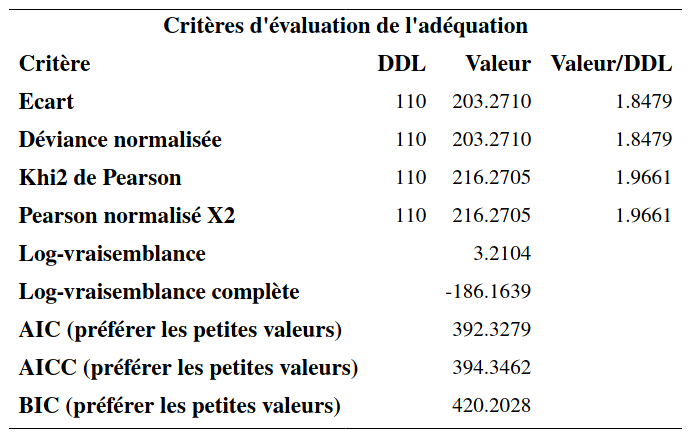
\includegraphics[width = 0.55\linewidth]{img/c4/diapos8-e3}
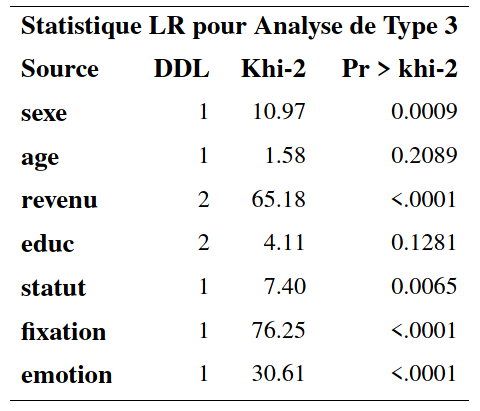
\includegraphics[width = 0.5\linewidth]{img/c4/diapos8-e4}
\end{center}
Cinq variables explicatives ont un effet non-nul selon les tests du rapport de vraisemblance.
\end{frame}


\begin{frame}[fragile]
\frametitle{Estimés des paramètres du modèle de Poisson}
\begin{center}
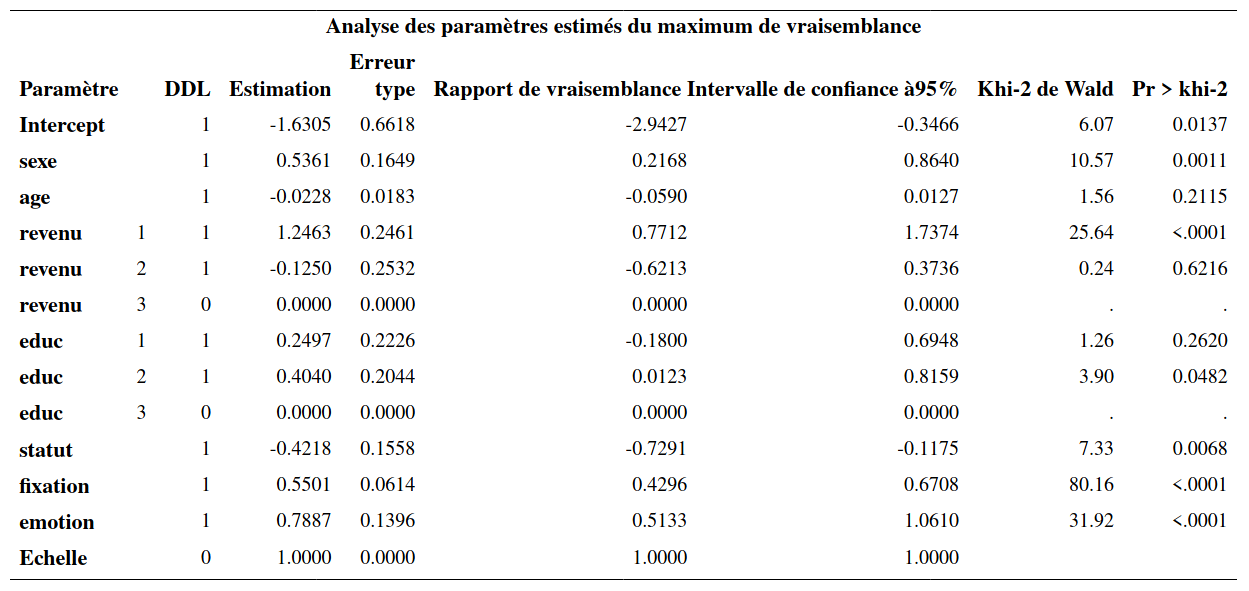
\includegraphics[width = 0.99\linewidth]{img/c4/diapos8-e5}
\end{center}
{\footnotesize
Le paramètre d'échelle est un parce que la variance est complètement déterminée par le modèle pour la moyenne.

}
\end{frame}

\begin{frame}[fragile]
\frametitle{Interprétation des paramètres significatifs}
\bi
\item Les femmes font plus d'achat, en moyenne, que les hommes. Lorsque les autres
variables demeurent fixes, la moyenne du nombre d'achats des femmes est
$\exp(0,5361) = 1,71$ fois celle des hommes. Ainsi, le nombre d'achats moyen
des femmes augmente de $71$\% par rapport à  celle des hommes.
\item L'estimé du paramètre de \texttt{fixation} est $\hat{\beta}_{\code{fixation}}=0,55$. Plus le temps de \texttt{fixation} augment, plus le nombre moyen d'achat est
élevé. Toutes choses étant égales par ailleurs, augmenter
\texttt{fixation} de un multiplie la moyenne du nombre d'achat par $\exp(0,55) =
1,73$.
\item \textit{Ceteris paribus}, le nombre moyen d'achat dans la catégorie à faible revenu achètent en moyenne $3,47$ fois plus que ceux dont le revenu est élevé, une augmentation moyenne de $247$\%.
\ei
\end{frame}
\begin{frame}
 \frametitle{Qualité de l'ajustement}
 {\small 
\bi \item  La sortie SAS inclut un tableau qui contient la valeur de la log-vraisemblance (log-vraisemblance complète) et les critères d'information. 
\item Pour le modèle de régression de Poisson, deux statistiques, la déviance et la statistique $X^2$ de Pearson, servent à mesurer la qualité de l'ajustement et à déterminer si le modèle est adéquat.
\ei
}
\begin{center}
 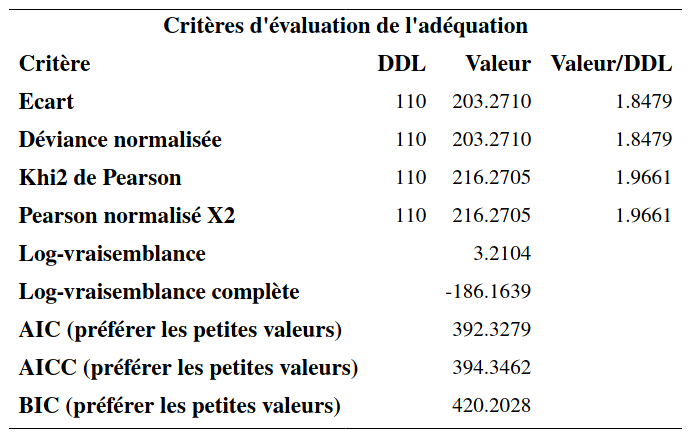
\includegraphics[width = 0.7\linewidth]{img/c4/diapos8-e3}
 \end{center}
 {\tiny
 Les premières lignes sont dupliquées; c'est dû au fait que la variance du modèle de Poisson est complètement déterminée par la moyenne.
 
 }
\end{frame}
\end{document}
